\section{Ablations}
\label{sec:ablations}

We run two ablations. The first sweeps the regularizer strength $\lambda$ to characterize the trade-off between geometric reshaping and retrieval. The second compares alternative placements of the regularizer to isolate which part of the token manifold is the operative target.

\subsection{Lambda Sweep}
\label{sec:ablations-lambda}

Table~\ref{tab:lambda} reports retrieval and geometry for $\lambda \in \{0, 0.1, 0.5\}$ as three-seed means under the same training protocol used in Section~\ref{sec:results}. Geometry shifts monotonically with $\lambda$. Intra-cosine on Spanish tokens drops from $0.2937$ at $\lambda=0$ to $0.2535$ at $\lambda=0.1$ to $0.1808$ at $\lambda=0.5$. Effective rank on Spanish climbs from $101.7$ to $103.8$ to $106.7$ over the same range. The regularizer continues to reshape the embedding manifold as we increase its weight.

Retrieval P@1 also improves monotonically but with diminishing returns. On EN-SW, the gain is $+3.25$ percentage points from $\lambda=0$ to $\lambda=0.1$, and an additional $+0.20$ percentage points from $\lambda=0.1$ to $\lambda=0.5$. On EN-AR, the gain is $+1.51$ percentage points then $+0.48$ percentage points. We read this as evidence that once anisotropy is no longer the bottleneck, further geometric pressure produces diminishing retrieval gains.

\begin{table}[t]
\centering
\caption{Effect of regularizer strength $\lambda$. Three-seed mean values for EN-SW P@1, EN-AR P@1, intra-cosine on Spanish tokens, and effective rank on Spanish tokens. Geometric metrics improve monotonically; retrieval payoff saturates near $\lambda=0.5$. \textit{Reproducibility note:} the $\lambda=0$ (vanilla) and $\lambda=0.5$ (IsoColBERT) columns are produced by the submitted multi-seed training notebook; the $\lambda=0.1$ column is from a prior 3-seed run conducted under the identical protocol (same architecture, optimizer, batch size, step count, and seed set), included here to characterize the trade-off curve.}
\label{tab:lambda}
\small
\begin{tabular}{lccc}
\toprule
Metric             & Vanilla & $\lambda{=}0.1$ & $\lambda{=}0.5$ \\
\midrule
EN--SW P@1         & $0.8344$ & $0.8669$ & $\mathbf{0.8689}$ \\
EN--AR P@1         & $0.9423$ & $0.9574$ & $\mathbf{0.9622}$ \\
Intra-cos ES $\downarrow$ & $0.2937$ & $0.2535$ & $\mathbf{0.1808}$ \\
eRank ES $\uparrow$       & $101.73$ & $103.78$ & $\mathbf{106.70}$ \\
\bottomrule
\end{tabular}
\end{table}

We select $\lambda = 0.5$ as the headline configuration in Section~\ref{sec:results-retrieval} because it produces the strongest geometric reshaping while remaining within the retrieval-improvement plateau on the low-resource pairs.

\subsection{Mechanism Ablation}
\label{sec:ablations-mechanism}

The uniform regularizer in \eqref{eq:reg} applies pressure to every pair of valid token vectors in the batch. Two natural alternatives restrict the regularization to a subset of tokens or move it from embeddings to matching scores. We compare three placements (each trained with $3$ seeds) to isolate which part of the token manifold is the operative target.

\paragraph{Active-token regularization.} For each query token, MaxSim selects one document token via the argmax in \eqref{eq:maxsim}. The active-token variant regularizes only the query tokens and their selected document tokens, applying \eqref{eq:reg} to the active subset rather than the full token bank.

\paragraph{Cross-attention regularization.} Rather than penalizing redundancy among embedding directions, the cross-attention variant penalizes redundancy among matching patterns. We treat the $L_q \times L_d$ matrix of pairwise similarities as a soft attention map (row-softmaxed across document tokens) and penalize squared off-diagonal correlations between rows. The intuition is to discourage different query tokens from attending to the same document token in similar ways.

\paragraph{Results.} Table~\ref{tab:mechanism} and Figure~\ref{fig:ablation} report the comparison. The uniform regularizer wins on every metric. EN-SW P@1 drops by $2.07$ percentage points under active-token regularization and by $3.68$ percentage points under cross-attention regularization. Intra-cosine on Spanish stays elevated under both alternatives ($0.24$ and $0.30$ vs.\ $0.18$ for uniform). Effective rank on Spanish recovers less ($104.2$ and $101.9$ vs.\ $106.7$).

\begin{table}[t]
\centering
\caption{Mechanism ablation. Three placements of the isotropy regularizer compared on EN-SW retrieval and ES token geometry. Numbers are 3-seed mean $\pm$ std. Uniform (the proposed IsoColBERT objective) strictly outperforms the localized and matching-level alternatives.}
\label{tab:mechanism}
\footnotesize
\setlength{\tabcolsep}{3pt}
\begin{tabular}{lccc}
\toprule
Placement     & EN--SW P@1 & I-cos ES $\downarrow$ & eRank ES $\uparrow$ \\
\midrule
Uniform (ours) & $\mathbf{.869 {\scriptstyle \pm.023}}$ & $\mathbf{.181 {\scriptstyle \pm.002}}$ & $\mathbf{106.7 {\scriptstyle \pm.5}}$ \\
Active-token   & $.848 {\scriptstyle \pm.013}$ & $.239 {\scriptstyle \pm.010}$ & $104.2 {\scriptstyle \pm.8}$ \\
Cross-attn.    & $.832 {\scriptstyle \pm.033}$ & $.299 {\scriptstyle \pm.006}$ & $101.9 {\scriptstyle \pm.2}$ \\
\bottomrule
\end{tabular}
\end{table}

\begin{figure*}[t]
\centering
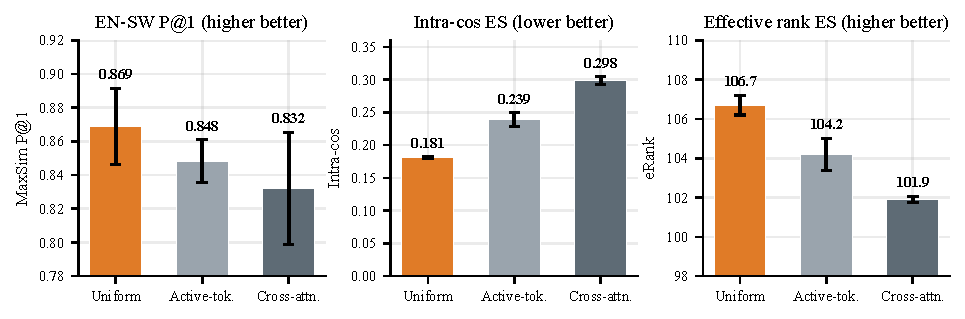
\includegraphics[width=\textwidth]{figs/fig_ablation.pdf}
\caption{Mechanism ablation: regularizing all valid tokens (uniform) outperforms regularizing only MaxSim-winning tokens (active-token) and regularizing the matching score matrix (cross-attention) on EN-SW retrieval and on both geometric metrics. 3-seed mean with $\pm$ standard deviation error bars.}
\label{fig:ablation}
\end{figure*}

\paragraph{Interpreting the localized result.} One reading of why active-token regularization underperforms: it only constrains tokens that already win MaxSim, leaving the losing alternatives unconstrained. If retrieval errors are driven by confusion among the losing tokens, this regularization surface would not directly address them. We caution that this is a post-hoc reading of a single experimental comparison rather than a tested causal mechanism; it is consistent with our results but does not establish that the active-token failure mode is exactly the one described.

\paragraph{Interpreting the object-level result.} A plausible reading of the cross-attention result is that the matching score matrix is a derivative quantity computed from the token vectors, and pushing the rows of the score matrix to be uncorrelated need not make the underlying token vectors more isotropic. Consistent with this reading, the cross-attention variant leaves intra-cosine and effective rank on Spanish near the vanilla baseline ($0.30$ vs.\ vanilla $0.29$; eRank $101.9$ vs.\ vanilla $101.7$) and recovers no retrieval gain. As above, this is a candidate explanation rather than a tested mechanism.

The empirical conclusion we draw from this ablation is narrower than ``broad embedding-space shaping is the mechanism.'' What we can say is that on this benchmark and backbone, of the three placements we tested, only the uniform variant produces both the geometric reshaping and the retrieval gain; the two restricted variants do not substitute for it. Whether other placements (regularizing only document tokens, restricting to a percentile of tokens, or different attention-style targets) could match or exceed uniform regularization remains open.
